\documentclass[a4paper,11pt]{jsarticle}
\renewcommand{\tablename}{Table }
\renewcommand{\figurename}{Fig.}

% 数式
\usepackage{amsmath,amsfonts}
\usepackage{bm}
% 画像
\usepackage[dvipdfmx]{graphicx}
\bibliographystyle{myjunsrt}
\renewcommand{\bibname}{References}


\begin{document}

\title{}
\author{}
\date{\today}
\maketitle

\section{Introduction}

The fifth generation (5G) mobile communication system
is expected to provide new innovations to support the society
with technical features including high speed, high
capacity, low latency, and massive connectivity.
As a special
feature of 5G, high frequency bands such as the millimeter
wave bands are supported to achieve ultra-high speed
wireless data communications of several gigabits per second
using a frequency bandwidth of
several-hundred megahertz \cite{docomo_6G_white_paper}.

However, propagation losses in line-of sight (LOS) and
performance degradation in non-line-of-sight (NLOS)
environments are crucial issues for mobile communication
systems in the millimeter wave bands. 
Solutions such as beamforming and
beam steering techniques employing array antenna systems
can mitigate these issues, and are
already implemented in 5G base station tools.
\cite{https://doi.org/10.48550/arxiv.2001.05021}

\section{Security}

In a hostile environment, the adversary's antenna can pick up signals from the
transmitter when the SNR at the antenna of the adversary is high enough.
In case of an omni-directional antenna, it can have a coverage of 360 degrees
and send data in all directions horizontally.
This can be both a waste of power and network capacity,
and can allow hostile devices to detect the radiated signals \cite{security_estimation_model}.
Therefore, using directive antennas, which form directional beams towards the receiver,
can be considered to be more safe.

\section{Mathematical analysis of waveguides}

Waveguides are devices for transporting electromagnetic energy
from one region to another.
There are a variety of waveguides, from hollow tubes made out of metal to
sticks made of teflon.
First we analyze waveguides that are hollow metal tubes
(often rectangular or circular in cross section).
These waveguides are capable of directing power precisely to where it is needed,
can handle large amounts of power and function as a high-pass filter.

\begin{figure}
  \begin{center}
    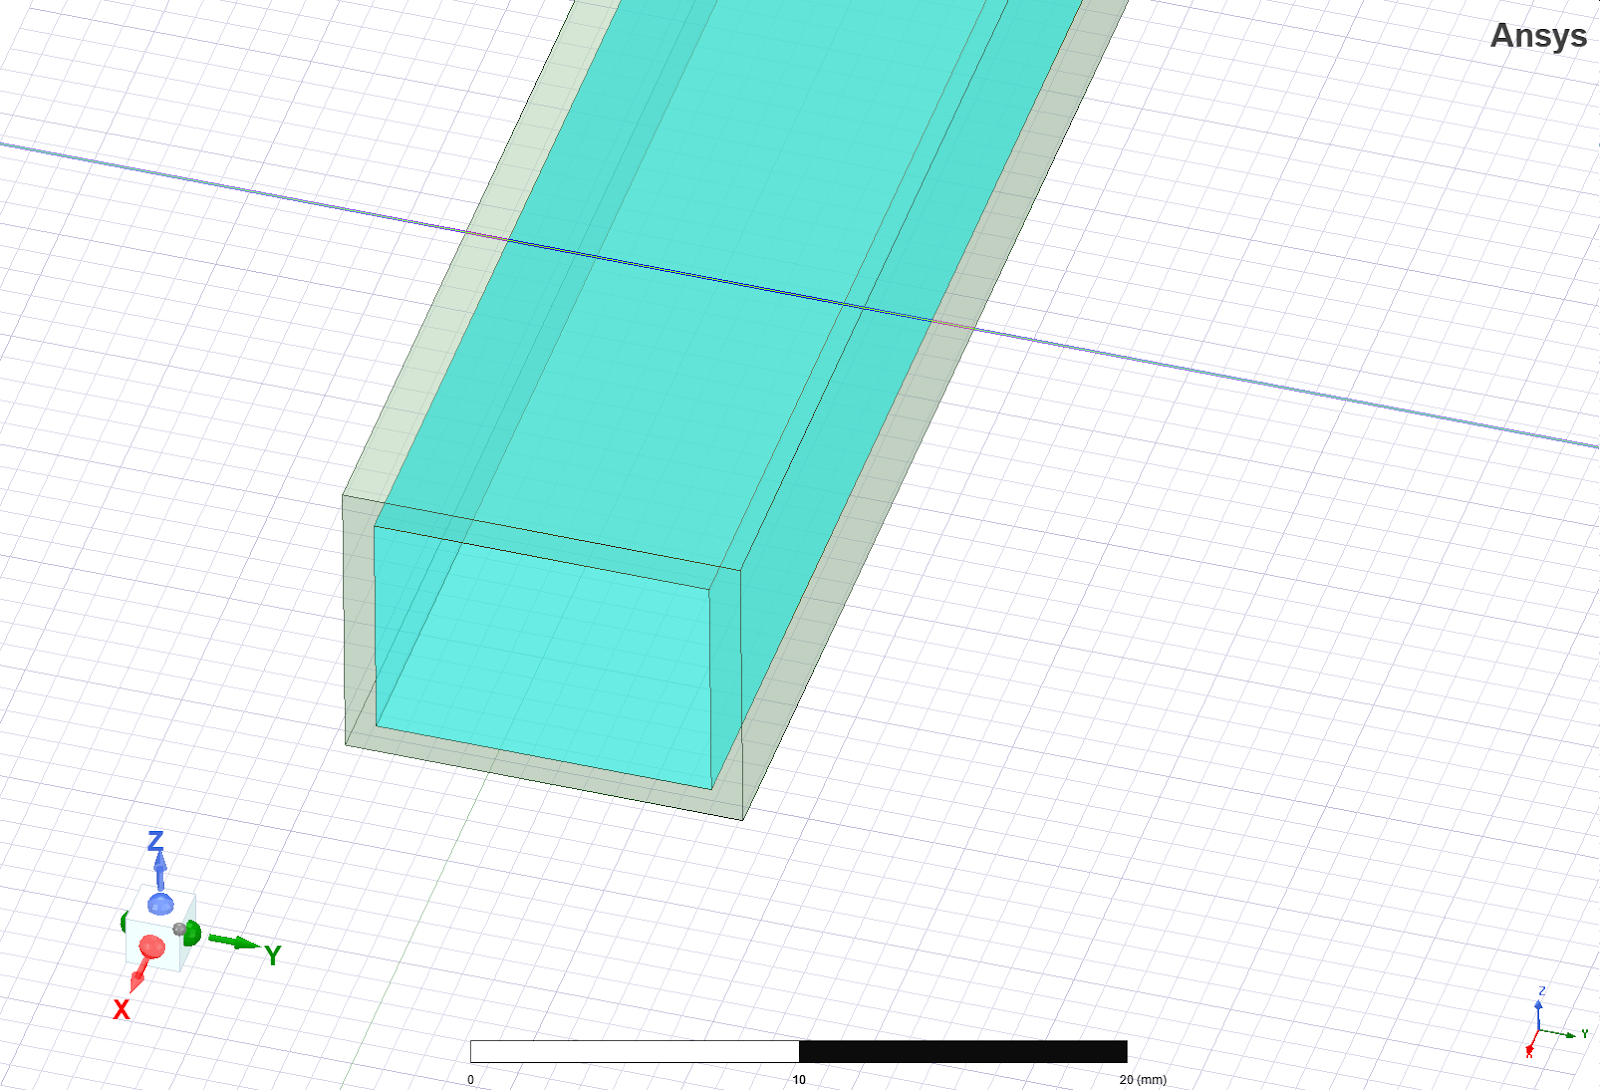
\includegraphics[clip, keepaspectratio, width=0.5\linewidth]{img/metal_waveguide.png}
    \caption{Model of metal waveguide}
    \label{fig:metal_waveguide}
  \end{center}
\end{figure}

Here we examine metal waveguides with a rectangular cross section.
In a source-free region, it is known that

\begin{equation}
  \nabla D = 0
\end{equation}

where $D$ is the electric flux density.
If a vector quantity is divergenceless,
then it can be expressed as the curl of another quantity.
The solution for $D$ and the corresponding electric field $E$
can be written as:

\begin{equation}
  D = -\nabla \times F
\end{equation}

\begin{equation}
  E = \frac{-1}{\epsilon}\nabla \times F
\end{equation}

where $\epsilon$ is the permittivity of the medium where the wave propagates.
Here for simplicity, it is assumed that $E_z$ is zero.
The following equations describing the electric and magnetic fields can be derived from Maxwell's equations.

\begin{equation}
  E_x = -\frac{1}{\epsilon}\frac{\partial F_z}{\partial y}
\end{equation}

\begin{equation}
  E_y = \frac{1}{\epsilon}\frac{\partial F_z}{\partial x}
\end{equation}

\begin{equation}
  E_z = 0
\end{equation}

\begin{equation}
  H_x = -j\frac{1}{\omega\mu\epsilon}\frac{\partial^2F_z}{\partial x \partial z}
\end{equation}

\begin{equation}
  H_y = -j\frac{1}{\omega\mu\epsilon}\frac{\partial^2F_z}{\partial y \partial z}
\end{equation}

\begin{equation}
  H_z = -j\frac{1}{\omega\mu\epsilon}(\frac{\partial^2}{\partial z^2} + k^2)F_z
\end{equation}

Here, $k$ is the wave number.
If the $F_z$, which is the z-axis component of the vector $F$, is found,
then the electric and magnetic fields can be found.
From Maxwell's equations, the vector potential $F$ must satisfy the vector wave equation
in a source-free region.

\begin{equation} \label{eq:vector_wave_equation}
  (\nabla^2 - \frac{1}{c^2}\frac{\partial^2}{\partial t^2})\boldsymbol{F} = 0
\end{equation}

Assuming that there is only one frequency, the time dependence can be written as

\begin{equation}
  e^{j\omega t} = e^{j 2\pi ft}
\end{equation}

Thus, the equation [\ref{eq:vector_wave_equation}] can be rewritten as follows:

\begin{equation} \label{eq:simplified}
  \nabla ^ 2 F_z + k^2 F_z = 0
\end{equation}

The technique of separation of variables is used to solve this equation.
It can be assumed that $F_z$ can be separated into the product of 3 functions.

\begin{equation} \label{eq:separation_of_vars}
  F_z(x,y,z) = X(x)Y(y)Z(z)
\end{equation}

Therefore, when equation [\ref{eq:separation_of_vars}] is plugged into equation [\ref{eq:simplified}],
the following equation is derived
(the prime represents the derivative):

\begin{equation} \label{eq:simplified_derivative_equation}
  \frac{X''}{X} + \frac{Y''}{Y} + \frac{Z''}{Z} = -k^2
\end{equation}

For simplicity, the wavenumber $k$ will be broken into components as below:

\begin{equation} \label{eq:break_down_wavenumber}
  k^2 = k_x^2 + k_y^2 + k_z^2
\end{equation}

Using equation [\ref{eq:break_down_wavenumber}] and the fact that all variables are
independent in equation [\ref{eq:simplified_derivative_equation}],
the followng ordinary differential equations are derived:

\begin{equation} \label{eq:three_ordinary}
  \left\{
  \begin{alignedat}{3}
    X'' + k_x^2 X = 0 \\
    Y'' + k_y^2 Y = 0 \\
    Z'' + k_z^2 Z = 0
  \end{alignedat}
  \right.
\end{equation}

Solving the above equations, we get:

\begin{equation} \label{eq:three_solved_ordinary}
  \left\{
  \begin{alignedat}{3}
    X(x) &= c_1 \cos (k_x x) + c_2 \sin (k_x x) \\
    Y(y) &= c_3 \cos (k_y y) + c_4 \sin (k_y y) \\
    Z(z) &= c_5 e^{j k_z z} + c_6 e^{-j k_z z}
  \end{alignedat}
  \right.
\end{equation}

The variable $c_5$ can be eliminated as $0$,
since waves analyzed here are propagating in the +z direction.
Plugging in the solutions above, $F_z$ can be written as

\begin{equation}
  F_z = [c_1 \cos (k_x x) + c_2 \sin (k_x x)][c_3 \cos (k_y y) + c_4 \sin (k_y y)]c_6 e^{-j k_z z}
\end{equation}

Using the condition that tangential electric fields in perfect conductors must be zero,
$E_x$ must be zero when $y=0$ and $y=b$.
The same could be said for $E_y$,
which is also zero when $x=0$ and $x=a$.
$E_x$ can be calculated as:

\begin{equation}
  \begin{split}
    E_x &= -\frac{1}{\epsilon} \frac{\partial F_z}{\partial y} \\
        &= - \frac{c_6 k_y}{\epsilon}[c_1 \cos (k_x x) + c_2 \sin (k_x x)][-c_3 \sin (k_y y) + c_4 \cos(k_y y)]e^{-jk_z z}
  \end{split}
\end{equation}

The boundary condition for $E_x$ is given by:

\begin{equation}
  E_x(x, y=0, z) = 0
\end{equation}

This implies that $c_4$ must be equal to zero.
As for the second boundary condition,

\begin{equation}
  E_x(x, y=b, z) = 0
\end{equation}

This means that $c_3 \sin (k_y b) = 0$, which means that the wavenumber $k_y$
can be written as follows:

\begin{equation} \label{eq:wavenumber_y}
  k_y = \frac{n\pi}{b}
\end{equation}

$n$ here is a natural number.
This states that the only solutions for $Y(y)$ function must be sinusoids,
and must have a wavenumber
which consists an integer number of multiples of a half-wavelength.
Simiarly in the y-axis, the following can be derived:

\begin{equation} \label{eq:wavenumber_x}
  k_x = \frac{m\pi}{a}
\end{equation}

This statement implies that the only functions of x that satisfy
the differential equation and the required boundary conditions
must be an integer multiple of half-sinusoids within the waveguide.
Combining these results, the solution for $F_z$ can be written as

\begin{equation}
  \begin{split}
    F_z &= A \cos(k_x x)\cos(k_y y)\exp(-j k_Z z) \\
        & = A \cos(\frac{m\pi x}{a}) \cos(\frac{n \pi y}{b})\exp(-j k_Z z)
  \end{split}
\end{equation}

Only certain distributions will satisfy the required differential equations
and the boundary conditions. These configurations are called modes.
Since this solution assumed that $E_z$ is zero, this mode is written as the $TE_{mn}$ mode.

Due to Maxwell's Equations,
the fields within the waveguide always have a specific "form" or "waveshape",
which are known as modes.
Assume the waveguide is oriented such that the energy is to be transmitted along the waveguide axis, the z-axis.
The modes are classified as either TE
('transverse electric' - which indicates that the E-field is orthogonal to the axis of the waveguide, so that Ez=0)
or TM ('transverse magnetic' - which indicates that the H-field is orthogonal to the axis of the waveguide, so Hz = 0).
The modes are further classified as $TE_ij$,
where the $i$ and $j$ indicate the number of wave oscillations for a particular
field direction in the long direction (dimension $a$ in Figure \ref{fig:metal_waveguide_geometry})
and short direction (dimension $b$ in Figure \ref{fig:metal_waveguide_geometry}), respectively.
Metal waveguides cannot support the TEM
('transverse electric and magnetic' - when Ez and Hz are zero) mode.
Their exists no solution to Maxwell's equations
that also satisfy the required boundary conditions for this mode to occur.

\begin{figure}
  \begin{center}
    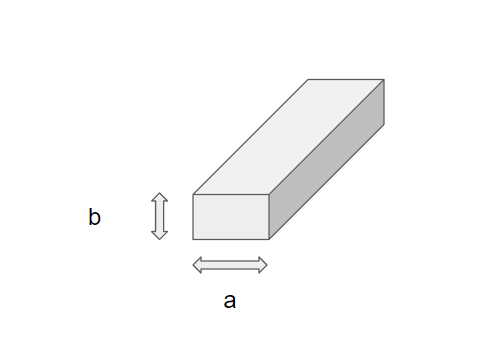
\includegraphics[clip, keepaspectratio, width=0.5\linewidth]{img/metal_waveguide_with_dims.png}
    \caption{Geometry of metal waveguide}
    \label{fig:metal_waveguide_geometry}
  \end{center}
\end{figure}

TODO: add from here https://www.antenna-theory.com/tutorial/waveguides/waveguides3.php

TODO add figure

\section{Horn Antennas}

Horn antennas are used in high frequency bands spanning from 300MHz
to even as high as 100GHz.
Horn antennas often have a directional radiation pattern with a high antenna gain,
which can range up to 25 dB in some cases, with 10-20 dB being typical.
Horn antennas have a wide impedance bandwidth,
implying that the input impedance is slowly varying over a wide frequency range (which also implies low values for S11 or VSWR). The bandwidth for practical horn antennas can be on the order of 20:1 (for instance, operating from 1 GHz-20 GHz),
with a 10:1 bandwidth not being uncommon.

https://www.antenna-theory.com/antennas/aperture/horn.php

TODO: add cross section of horn antenna in H-plane

TODO: add cross section of horn antenna in V-plane

The E-field in the far-field becomes linearly polarized.
The magnitude of the E-field can be written as:

\begin{equation}
  |E| = \frac{k}{4 \pi r}(1 + \cos(\theta))\int_{-B/2}^{B/2}\int_{-A/2}^{A/2}E_A(x,y)e^{jk(x\sin\theta\cos\phi + y\sin\theta\sin\phi)}dxdy
\end{equation}

This equation implies that the far-fields of the horn antenna
is the Fourier Transform of the fields at the opening of the horn.

TODO: copy here https://www.thefouriertransform.com/applications/radiation.php

Modeling the electric field as the magnetic surface current $M_S$,
it can be written as:

\begin{equation}
  M_S = E_a \times \hat{n}
\end{equation}

$\hat{n}$ is the unit vector perpendicular to the surface.
The electric fields $E$ and magnetic fields $H$ in the far field can be written as:

\begin{equation}
  E = \eta H \times \hat{r}
\end{equation}

\begin{equation}
  H = \hat{r} \times \frac{E}{\eta}
\end{equation}

Here, $\eta$ is the characteristic impedance of free space,
which is about 377 Ohms. $\hat{r}$ is the direction of propagation for the plane wave.

\begin{figure}
  \begin{center}
    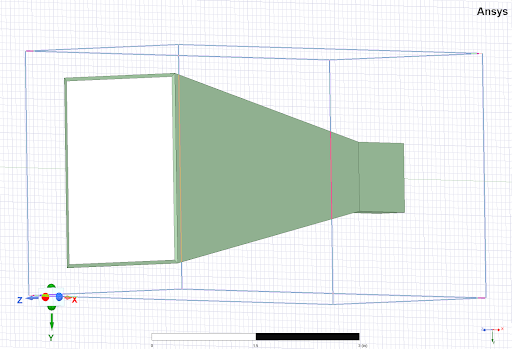
\includegraphics[clip, keepaspectratio, width=0.5\linewidth]{img/horn_antenna_model.png}
    \caption{Model of horn antenna}
    \label{fig:model_horn_antenna}
  \end{center}
\end{figure}

The waveguide feed acts as a high-pass filter,
which blocks any energy below its cutoff frequency.
The antenna gain is affected by the geometry of the horn antenna.

\section{Radar}

Radar works by transmitting an electromagnetic wave from an antenna.
The wave then bounces off some object, and the returned energy is measured.
The amount of energy returned is a function of the radar cross section of the object.

If we can estimate the fields radiated by an antenna,
we can estimate the surface electric current induced on an object
(such as an airplane).

\section{Antenna Gain}

The term antenna gain describes how much power is transmitted
in the direction of peak radiation to that of an isotropic source.
A transmitting antenna with a gain of 3 dB means that the power received
far from the antenna will be 3 dB higher (twice as much) than
what would be received from a lossless isotropic antenna with the
same input power. Note that a lossless antenna would be an antenna
with an antenna efficiency of 0 dB.
Similarly, a receive antenna with a gain of 3 dB in a particular direction
would receive 3 dB more power than a lossless isotropic antenna.
Antenna Gain is sometimes discussed as a function of angle.
In this case, we are essentially plotting the radiation pattern,
where the units (or magnitude of the pattern) are measured in antenna gain.
Often manufacturers of antennas
(be they wifi antennas, gps antennas, or tv antennas) specify the antenna gain.
For instance, manufacturers of wifi antennas may market the wifi antenna as a "high gain antenna",
which is more expensive than a similar low gain antenna.
Here we discuss how different devices have different gain,
as the need for high/low gain differs depends on the situation.

\begin{table}[h]
  \centering
  \caption{Comparisons of Preferred Gain}
  \label{table}
  \begin{tabular}[]{lcc}
    \hline
    Example & Preferred Gain & Reason \\
    \hline\hline
    TV antennas & High & Location of the broadcast antennas are known. \\
    \hline
    GPS & Low & Location of GPS satellites are unknown \\
    \hline
    Mobile Cellular Antennas & Low & Location of cell towers are unknown \\
    \hline
  \end{tabular}
\end{table}

\section{Antenna Impedance}


Antenna impedance relates the voltage to the current at the input to the antenna.
This is an important parameter to look out for when conducting experiments.

For instance, when an antenna has an impedance of 50 ohms,
this means that if a sinusoidal voltage is applied at the antenna terminals with an amplitude of 1 Volt,
then the current will have an amplitude of 1/50 = 0.02 Amps.
Since the impedance is a real number, the voltage is in-phase with the current.

Alternatively, when the impedance is given by a complex number,
the phase will need to be considered additionaly to the amplitude.
If impedance $Z$ is writen as $50 + j*50$, where $j$ is an imaginary number,
then the impedance has a magnitude equal to:

\begin{equation}
  \sqrt[]{50^2 + 50 ^2} = 70.71
\end{equation}

The phase can be calculated as:

\begin{equation}
  \tan^{-1}(\frac{Im(Z)}{Re(Z)}) = \frac{\pi}{4}
\end{equation}

The real part of the antenna impedance represents power that is either radiated away or absorbed within the antenna.
The imaginary part of the impedance represents power
that is stored in the near field of the antenna.
This is non-radiated power.
An antenna with a real input impedance (zero imaginary part)
is said to be resonant.

\subsection{Impedance in low frequencies}

When we are dealing with low frequencies,
the transmission line that connects the transmitter or receiver
to the antenna is short relative to the wavelength.

Consider an antenna which is represented as an impedance given by $Z_A$,
hooked up to a voltage source (of magnitude $V$) with source impedance given by $Z_s$.
The equivalent circuit of this is shown in
Figure \ref{fig:low_freq_circuit_diagram}.

\begin{figure}
  \begin{center}
    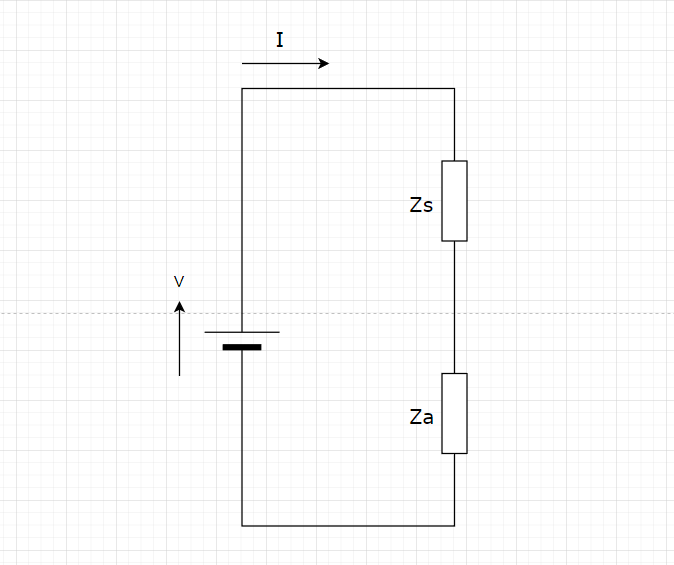
\includegraphics[clip, keepaspectratio, width=0.5\linewidth]{img/low_freq_circuit_diagram.png}
    \caption{Circuit model of antenna connected to voltage source}
    \label{fig:low_freq_circuit_diagram}
  \end{center}
\end{figure}

Using the equation $P=IV$ from circuit theory,
the power delivered to the antenna can be calculated as:

\begin{equation}
  P_A = \frac{V^2 Z_A}{(Z_A + Z_S) ^2}
\end{equation}

If $Z_A$ is much smaller in magnitude than $Z_S$,
then no power will be delivered to the antenna and
it won't transmit or receive energy.
The same can be said when $Z_A$ is much larger in magnitude than $Z_S$.
The ideal value for antenna impedance when maximum power is transferred is given as:

\begin{equation}
  Z_A = Z_S^*
\end{equation}

where $Z_S*$ is the complex conjugate of $Z_S$.
For example, if $Z_S = 30 + 30j$, then $Z_A = 30 - 30j$ is the ideal
impedance for maximum power transfer.

\subsection{Impedance in high frequencies}

In low-frequency circuit theory, the wires that connect things don't matter.
Once the wires become a significant fraction of a wavelength,
the situation changes. For instance,
a short circuit has an impedance of zero ohms. However,
if the impedance is measured at the end of a quarter wavelength transmission line,
the impedance appears to be infinite,
even though there is a direct current conduction path.

In general, the transmission line will transform the impedance of an antenna,
making it very difficult to deliver power,
unless the antenna is matched to the transmission line.
Consider the situation shown in Figure \ref{fig:high_freq_circuit_diagram}.
The impedance is to be measured at the end of a transmission line
(with characteristic impedance $Z_0$) and Length $L$.
The end of the transmission line is hooked to an antenna with impedance $Z_A$.

\begin{figure}
  \begin{center}
    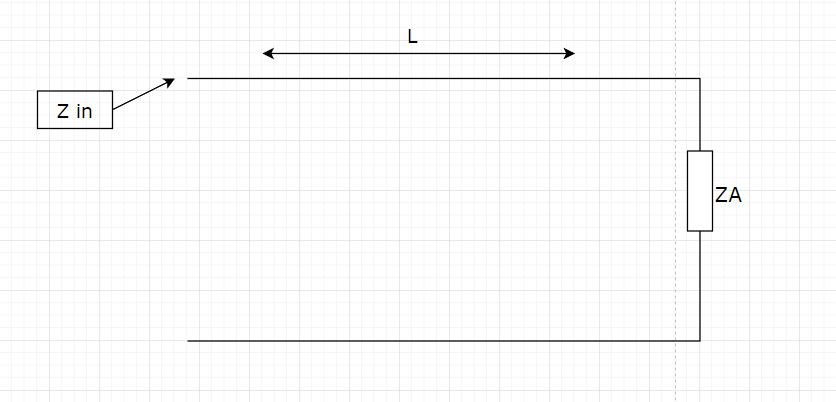
\includegraphics[clip, keepaspectratio, width=0.5\linewidth]{img/high_freq_circuit_diagram.png}
    \caption{High frequency circuit model}
    \label{fig:high_freq_circuit_diagram}
  \end{center}
\end{figure}

Input impedance $Z_in$ is given by:

\begin{equation}
  Z_{in} = Z_0 \frac{Z_A + j Z_0 \tan(\frac{2\pi f}{c}) L}{Z_0 + j Z_A \tan(\frac{2\pi f}{c}) L}
\end{equation}

If the antenna is matched to the transmission line ($Z_A=Z_0$),
then the input impedance does not depend on the length of the transmission line.

If the antenna is not matched,
the input impedance will vary widely with the length of the transmission line.
And if the input impedance isn't well matched to the source impedance,
not very much power will be delivered to the antenna.
This power ends up being reflected back to the generator,
which can be a problem in itself (especially if high power is transmitted).
This loss of power is known as impedance mismatch.
Hence, having a tuned impedance for an antenna is extremely important.

\section{The Friis Equation}

One of the most fundamental equations in antenna theory is the Friis Transmission Equation.
The Friis Transmission Equation is used to calculate the power
received from one antenna
(with gain $G1$), when transmitted from another antenna (with gain $G2$),
separated by a distance $R$, and operating at frequency $f$ or wavelength $\lambda$. 
The two antennas are considered to be in free space.

\begin{figure}
  \begin{center}
    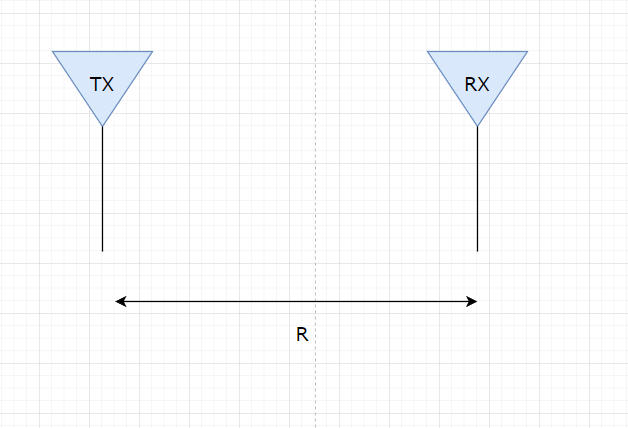
\includegraphics[clip, keepaspectratio, width=0.5\linewidth]{img/friis_equation.png}
    \caption{Transmit (Tx) and Receive (Rx) Antennas separated by R.}
    \label{fig:friis_equation}
  \end{center}
\end{figure}

Assume that $P_T$ watts of total power are delivered
to the transmit antenna and that the transmit antenna is omnidirectional, lossless,
and that the receive antenna is in the far field of the transmit antenna.
Then the power density $p$ (in Watts per square meter)
from the transmit antenna is given by:

\begin{equation}
  p = \frac{P_T}{4\pi R^2}
\end{equation}

If the transmit antenna has an antenna gain
in the direction of the receive antenna given by $G_T$,
then the power density can be written as:

\begin{equation}
  p = \frac{P_T}{4\pi R^2} G_T
\end{equation}

The gain term factors in the directionality and losses of a real antenna.
Assume now that the receive antenna has an effective aperture given by $A_ER$.
Then the power received by this antenna $P_R$ is given by:

\begin{equation}
  p = \frac{P_T}{4\pi R^2} G_T A_ER
\end{equation}

Since the effective aperture for any antenna can also be expressed as:

\begin{equation}
  A_e = \frac{\lambda ^ 2}{4 \pi} G
\end{equation}

Plugging in this result, the received power can be rewritten as:

\begin{equation} \label{eq:friis_transmission_formula}
  p = \frac{P_T G_T G_R \lambda^2}{(4\pi R)^2}
\end{equation}

Equation \ref{eq:friis_transmission_formula} is the
Friis Transmission Formula, and relates the free space path loss,
antenna gains and wavelength to the received and transmit powers.

When we plug in the wave equation $c = f\lambda$,
where $c$ is the speed of light, $f$ is the frequency,
and $lambda$ is the wavelength, we get:

\begin{equation} \label{eq:friis_transmission_formula_ver2}
  P_R = \frac{P_T G_T G_R c^2}{(4\pi R f)^2}
\end{equation}

Equation \ref{eq:friis_transmission_formula_ver2}
shows that more power is lost at higher frequencies.
This means that for antennas with specified gains,
the energy transfer will be highest at lower frequencies.
The difference between the power received and
the power transmitted is known as path loss.

Using \ref{eq:friis_transmission_formula},
loss $L$ (in decibels) in free space can be rewritten as follows:

\begin{equation}
  L = \left(\frac{4\pi d}{\lambda} \right)^2
\end{equation}

At 28GHz, which has the wave length of 10mm,
the loss at the distance of 0.25cm can be computed as -49.3 decibels.
At 800MHz (wave length of 375mm), the same loss of -49.3 decibels can be seen at
the distance of 10 meters.

\section{Loss tangent}

In a dielectric material, dielectric loss quantifies the inherent dissipation
of electromagnetic energy, and can be parametrized in terms of the loss tangent.
The basic equation for electromagnetic waves
when there is loss in the medium is as follows

\begin{equation}
  \mathrm{rot}(\frac{1}{\mu(\boldsymbol{r})}\mathrm{rot}\boldsymbol{E}) = -\mu_0 \mathrm{rot}(\frac{\partial H}{\partial t})
\end{equation}
\begin{equation}
  \mathrm{rot}(\frac{\partial H}{\partial t}) = \epsilon(\boldsymbol{r})\epsilon_0 \frac{\partial^2 E}{\partial t^2} + \frac{\partial J}{\partial t}
\end{equation}


We consider the characteristic value when there is loss in the medium.
When we consider the incidence of the time-varying factor $exp(j\omega t)$,
Maxwell's Equation can be written as follows.

\begin{equation} \label{eq:loss_electric_flux_density}
  \mathrm{rot} H = \epsilon \epsilon_0 \frac{\partial E}{\partial t} + \sigma \boldsymbol{E} = (j\omega\epsilon\epsilon_0 + \sigma)\boldsymbol{E}
\end{equation}

In this case, the right-hand side of Equation \ref{eq:loss_electric_flux_density}
is considered to arise from the flux density $\boldsymbol{D}$.

\begin{equation} \label{eq:electric_flux_density}
  \boldsymbol{D} = C\epsilon \epsilon_0 \boldsymbol{E}(\boldsymbol{r})exp(j\omega t)
\end{equation}

We derive the constant $C=1 - j\sigma / \omega\epsilon\epsilon_0$ from the equation above.
Thus the electric flux density can be written as

\begin{equation} \label{eq:electric_flux_density_tangent_delta}
  \boldsymbol{D} = \dot{\epsilon} \epsilon_0 \boldsymbol{E} = \epsilon \epsilon_0 (1 - j\tan\delta)\boldsymbol{E}
\end{equation}

\begin{equation} \label{eq:epsilon_dot}
  \dot{\epsilon} = \epsilon (1 - j\tan\delta)
\end{equation}

\begin{equation} \label{eq:tangent_delta}
  \tan \delta = \frac{\sigma}{\omega\epsilon\epsilon_0}
\end{equation}

The parameter in Eq. \ref{eq:tangent_delta} is known as the loss tangent.
At high frequencies, the contribution of the real part of $\epsilon$ becomes larger,
while at low frequencies, the contribution of the imaginary part becomes larger.
In other words, it can be said that when an AC electric field is applied to a dielectric,
a part of its energy is the ratio that becomes heat.

\section{Skin effect}

Skin effect is the tendency of an alternating current to flow mostly near
the outer surface of an electrical conductor, such as copper plates.
In many of the experiments in this study, 
millimeter waves are blocked by copper plates.
The conductivity of the conductor $\sigma$ increases,
and the amplitude damping constant $\alpha$ and the phase constant$\beta$
can be estimated as below.

\begin{equation}
  \alpha \approx \beta \approx \sqrt[]{\frac{\omega\mu\mu_0\sigma}{2}}
\end{equation}

This means that the attenuation of electromagnetic waves increases with increasing conductivity of $\sigma$
and the electromagnetic wave attenuates exponentially.
The depth δ at which the amplitude of the electromagnetic wave
at the surface is 1/e is called the skin depth, which can be expressed as below.

\begin{equation}
  \delta = \frac{1}{\alpha} = \sqrt[]{\frac{2}{\omega\mu\mu_0\sigma}}
\end{equation}

This indicates that the skin depth becomes shallower
as the frequency of the electromagnetic wave increases and the conductivity increases.
In this case, the current flows only near the surface of the copper plate,
which is called the skin effect.
The fact that current flows means that resistance exists,
and the skin resistance is written as follows.

\begin{equation}
  Re\{Z_W\} = \sqrt[]{\frac{\omega\mu\mu_0}{2}} = \frac{1}{\delta\sigma}
\end{equation}

Therefore copper plates can be used to effectively block millimeter waves.

\section{Snell's law}

At the boundary surfaces of different media, reflection and refraction of electromagnetic waves occur.
This is described by Snell's law.
This law can be derived using Maxwell's equations and boundary conditions.

The boundary plane of the medium is the x-y plane,
and the medium is uniform in the y direction within each region.
The relative permittivity and relative permeability are
$\dot{\epsilon_1}$ and $\mu_1$ for the first medium, and
$\dot{\epsilon_2}$ and $\mu_2$ for the second medium.
Let the complex permittivity in the presence of loss be
$i$ for each medium, so take values of 1 and 2, respectively.


\begin{equation}
  \dot{\epsilon_i} = \epsilon_i(1 - j\frac{\sigma_i}{\omega\epsilon_i\epsilon_0})
\end{equation}

Here $\sigma$ is the conductivity,
$\omega$ is the angular frequency of the electromagnetic wave,
$\epsilon$ is the dielectric constant when there is no loss, and
$\epsilon_0$ is the dielectric constant of vacuum.
The specific permeability $\mu$ is assumed to be a real number this time.
Here the magnitude of the wavenumber of each medium is as follows as $k$.
$c$ is the speed of light in vacuum.

\begin{equation}
  k_i = \frac{\omega\sqrt[]{\dot{\epsilon_i}\mu_i}}{c}
\end{equation}

Here we derive Snell's law using the TE wave as an example.
For TE waves,
the oscillation direction of the electric field is perpendicular to the surface,
and there is no electric field component in the direction of propagation.
Since the direction perpendicular to the surface is the y-axis,
its electric field is $E^i_y$ and can be written as follows:

\begin{equation}
  E^i_y = A_{iS}\exp[j(\omega t - \boldsymbol{k}_i\cdot\boldsymbol{r})]
\end{equation}

$A_{iS}$ is the electric field amplitude,
$\boldsymbol{k}_i$is the wavenumber vector in the medium, and
$\boldsymbol{r}$ is the position vector to an arbitrary point on the wavefront.
The subscript $i$ has three states,
where incident, transmitted, and reflected are denoted by i, t, and r, respectively.

\section{Total Reflection}

When an electromagnetic wave is incident on a sparse medium from a dense medium,
the refraction angle reaches 90 degrees before the incident angle
as the incident angle is gradually increased.
This phenomenon in which the incident electromagnetic wave
returns to the incident side after being reflected
at the boundary surface without being transmitted is called total reflection.

The transmitted field components of the TE wave at total reflection
can be written as follows.


\begin{equation}
  E^t_y = \exp[-j(\sqrt[]{\epsilon_1\mu_1}k_0\sin\theta_t)x]\exp\left(-\frac{z}{z_g}\right)
\end{equation}

\begin{equation}
  z_g = \frac{c}{\omega\sqrt[]{\epsilon_1\mu_1\sin^{2}\theta - \epsilon_2\mu_2}}
\end{equation}

$z_g$ represents the depth of penetration of the electric field into the second medium,
indicating that the electromagnetic wave is seeping slightly into the boundary surface.
Even during total reflection, 
electromagnetic waves also slightly penetrate to the other side of the boundary.
This component is called the evanescent wave.
Along with the penetration of the electromagnetic field,
the reflection point is also shifted.
This shift is called the Guschenchen shift.
This is important when using dielectric waveguides and optical fibers.


Electromagnetic waves do seep out slightly
to the other side of the boundary plane,
but it is important to note that the energy does not seep out.
It is important to note that energy does not seep out.
The sum of the amplitude reflection coefficients all add up to 1,
and all energy is also reflected.

\begin{figure}
  \begin{center}
    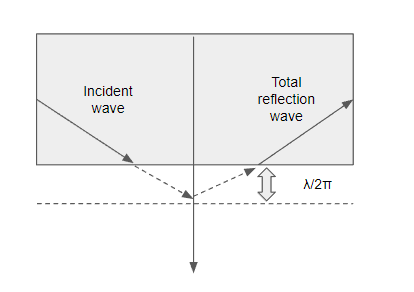
\includegraphics[clip, keepaspectratio, width=0.5\linewidth]{img/insertion_reflection_evanescence.png}
    \caption{Evanescent waves present in total internal reflection}
    \label{fig:insertion_reflection_evanescent}
  \end{center}
\end{figure}


\section{Link budget}

A link budget is an accounting of all of the power gains and losses
that a communication signal experiences in a telecommunication system;
from a transmitter, through a communication medium such as radio waves,
cable, waveguide, or optical fiber, to the receiver.
A simple link budget equation looks like this:

\begin{equation}
  RP = TP + Gain - Loss
\end{equation}

RP and TP are short for received power and transmitted power, respectively.
While RP and TP are in units of decibels-milliwatts, Gain and Loss are in units of decibels.

\section{Cutoff Frequency}

A cutoff frequency, corner frequency, or break frequency
is a boundary in a system's frequency response at which
energy flowing through the system begins to be reduced
rather than passing through.
This means that the signals with a frequency above the cut-off frequency
will travel through a waveguide and signals below this frequency
will be attenuated.

Using the fact that
the components of the wavenumber must satisfy the relationship:

\begin{equation}
  k_x^2 + k_y^2 + k_z^2 = \omega^2\mu\epsilon = \left(\frac{2\pi f}{c}\right)^2
\end{equation}

Assuming the situations are the same as
in the equations \ref{eq:wavenumber_y} and \ref{eq:wavenumber_x},
by plugging them in we get:

\begin{equation}
  \left(\frac{m\pi}{a}\right)^2 + \left(\frac{n\pi}{b}\right)^2 + k_z^2 = k^2 = \left(\frac{2\pi f}{c}\right)^2
\end{equation}

$k_z^2 > 0$ is the necessary condition for propagation to occur.
If this is true, then $k_z$ is a real number,
so that the field components will contain complex exponentials,
which represent propagating waves.
Otherwise when $k_z^2 < 0$,
$k_z$ will be an imaginary number,
in which case the complex exponential becomes a decaying real exponential.
In this case, the fields will not propagate but instead quickly die out within the waveguide.
Electromagnetic fields that die off instead of propagate are referred to as evanescent waves.

TODO add here https://www.antenna-theory.com/tutorial/waveguides/waveguides3.php

Cutoff frequency $f_c$ in a rectangular waveguide can be calculated as follows,
where $a$ is the wall length, and $\mu$ and $\epsilon$ are
the permeability and permittivity of the material
that fill the waveguide, respectively.

\begin{equation}
  f_c = \frac{1}{2a\sqrt[]{\mu\epsilon}}
\end{equation}

In a circular waveguide with radius of $a$,
$f_c$ could be written as

\begin{equation}
  f_c = \frac{1.8412}{2\pi a\sqrt[]{\mu\epsilon}}
\end{equation}

\section{Related Work}

In millimeter wave bands, Kawai et al. have proposed an approach that expands
communication areas by using a flexible dieletric waveguide,
wchich has low loss characteristics in the millimeter wave band range \cite{new_area_formation_approach}.
Fukuda et al. have proposed a leaky-wave antenna employing a bent dielectric waveguide for
millimeter wave bands \cite{leaky_wave_antenna_bent_dielectric}.
The study utilizes the characteristics that the
dielectric waveguide radiates electromagnetic waves by
inflection, and that the inflected part of the waveguide acts as
an antenna.
Since
the inflected part can be formed anywhere along the length of
the waveguide, it is possible to expand communication areas
around the waveguide. 
Antenna gain values of 3 dB to 5 dB are
achieved in both H-plane and V-plane,
and a narrow beam was created in the V-plane.

\section{Usecases}

This approach show the advantages in the following aspects compared to
other communication mediums.

\begin{enumerate}
  \item \textbf{Cost efficiency} Flexible
  dielectric waveguides are cheaper compared to SMA cables and horn antennas.
  The length and radius of the PTFE sticks can be also adjusted easily.
  \item \textbf{Flexibility} Flexible dielectric waveguides can be bent
  flexibly, unlike horn antennas, which make them suitable in environments
  with less space.
  \item \textbf{Low propagation loss} Compared to SMA cables, dielectric waveguides
  have less loss when propagating signals in the millimeter wave bands.
\end{enumerate}

The high resolution beam from the dielectric waveguide
enables users and devices to create an one to one
connection with the access point.
From the perspective of security, this eliminates the possibility of
malicious devices spying on the electromagnetic signals emitted from the device.

This approach allows the users and their devices to create a
secure connection in the physical layer.
Numerous studies have been done on the software side to protect the
data communicated between the device and the access point by using
encryption algorithms, such as AES.
Our approach is different from previous studies
in the sense that secure communication zones are created in the physical world.

This approach can be used in offices where employees handle
vital information that cannot be leaked, and in places such as ATMs,
where customers often look up important information on their
smartphones before making transactions from their bank accounts.

\section{Two Dimensional Waveguide Sheets}

\section{Finite Element Boundary Integral Method}

The finite element boundary integral method
combines the finite element
method (FEM) and the surface integral equation
embodied in the extended boundary condition
method (EBCM).

The theory of the extended boundary condition
method is well known and only the equations
which are required for the extension of the technique to the inhomogeneous problem will be given
here.
Consider a scatterer illuminated by a plane
wave. The incident field $\bar{E_i}$ and the scattered field
$\bar{E_s}$, can be expanded in the spherical vector harmonics $\bar{M}$ and $\bar{N}$.

\begin{equation}
  \bar{E_i} = \sum_{\nu}D_{\nu}[a_{\nu}\bar{M}_{\nu}^1(k_0\bar{r})+b_{\nu}\bar{N}_{\nu}^1(k_0\bar{r})]
\end{equation}

\begin{equation}
  \bar{E_s} = \sum_{\nu}D_{\nu}[f_{\nu}\bar{M}_{\nu}^4(k_0\bar{r})+g_{\nu}\bar{N}_{\nu}^4(k_0\bar{r})]
\end{equation}

The $a_{\nu}$ and $b_{\nu}$ coefficients are known, while $f_{\nu}$ and
$q_{\nu}$, are initially unknown. $D_{\nu}$ is a normalization
constant, $\nu$ is a combined index incorporating tht
three spherical harmonic indices. and $k_0$ is the free space wave number.

TODO: write rest https://core.ac.uk/download/pdf/36739115.pdf

\section{Directivity Results}

\newpage
\addcontentsline{toc}{chapter}{\bibname}
\bibliography{common_bibliography}

\end{document}